\subsection{Experiment \rnum{2}: Anomaly Detection}

Table \ref{tab:confusion-matrix-results} presents a comparative analysis of all four models and data types. Except for the $\beta$-VAE model, all scores are equal between all metrics. The variational models have the highest values for the positives and the lowest of the negatives. The CAE model has a higher rate of falsely predicted values, yet still close to the variational ones.

\begin{table}[!htbp]
\centering
\begin{tabular}{l cccccccc}
\toprule
\multirow{2}{*}{\textbf{Model}} & \multicolumn{2}{c}{\textbf{TP}} & \multicolumn{2}{c}{\textbf{FP}} & \multicolumn{2}{c}{\textbf{TN}} & \multicolumn{2}{c}{\textbf{FN}} \\
\cmidrule(lr){2-3} \cmidrule(lr){4-5} \cmidrule(lr){6-7} \cmidrule(lr){8-9}
& \textbf{F32} & \textbf{F16} & \textbf{F32} & \textbf{F16} & \textbf{F32} & \textbf{F16} & \textbf{F32} & \textbf{F16} \\
\midrule
\rowcolor{gray!10} AE   & 0 & 0 & 42 & 42 & 418 & 418 & 140 & 140 \\
$\beta$-VAE  & 109 & 105 & 13 & 7 & 447 & 453 & 31 & 35 \\
\rowcolor{gray!10} CAE  & 96 & 96 & 10 & 10 & 450 & 450 & 44 & 44 \\
$\beta$-CVAE & 106 & 106 & 9 & 9 & 451 & 451 & 34 & 34 \\
\bottomrule
\end{tabular}
\caption{Confusion Matrix Values for all four models and datatypes (Float32 and Float16)}
\label{tab:confusion-matrix-results}
\end{table}

Table \ref{tab:performance-metrics-float32} highlights the key metrics when we use Float32 for anomaly detection. Except for the AE model, all models score above 90\% on accuracy, prediction, and F1-score with a low FPR.

\begin{table}[!htbp]
\centering
\begin{tabular}{l
    S[table-format=1.3]
    S[table-format=1.3]
    S[table-format=1.3]
    S[table-format=1.3]
    S[table-format=1.3]
    S[table-format=1.3]
    S[table-format=1.3]
}
\toprule
\textbf{Model} & {\textbf{Accuracy}} & {\textbf{Precision}} & {\textbf{Recall}} & {\textbf{F1-Score}} & {\textbf{FPR}} & {\textbf{ROC AUC}} & {\textbf{PR AUC}} \\
\midrule
\rowcolor{gray!10} AE   & 0.697 & 0.000 & 0.000 & 0.000 & 0.091 & 0.292 & 0 \\
$\beta$-VAE  & 0.927 & 0.893 & 0.779 & 0.832 & 0.028 & 0.968 & 0 \\
\rowcolor{gray!10} CAE  & 0.910 & 0.906 & 0.686 & 0.780 & 0.022 & 0.843 & 0 \\
$\beta$-CVAE & 0.928 & 0.922 & 0.757 & 0.831 & 0.020 & 0.967 & 0 \\
\bottomrule
\end{tabular}
\caption{Anomaly Detection Performance Metrics Comparison (Float32)}
\label{tab:performance-metrics-float32}
\end{table}

Like Table \ref{tab:performance-metrics-float32}, Table \ref{tab:performance-metrics-float16} scores high on the same metrics. Only the $\beta$-VAE scores differ between single-precision and half-precision metrics.
\begin{table}[!htbp]
\centering
\begin{tabular}{l
    S[table-format=1.3]
    S[table-format=1.3]
    S[table-format=1.3]
    S[table-format=1.3]
    S[table-format=1.3]
    S[table-format=1.3]
    S[table-format=1.3]
}
\toprule
\textbf{Model} & {\textbf{Accuracy}} & {\textbf{Precision}} & {\textbf{Recall}} & {\textbf{F1-Score}} & {\textbf{FPR}} & {\textbf{ROC AUC}} & {\textbf{PR AUC}} \\
\midrule
\rowcolor{gray!10} AE   & 0.697 & 0.000 & 0.000 & 0.000 & 0.091 & 0.293 & 0.233 \\
$\beta$-VAE  & \textbf{0.930} & \textbf{0.938} & 0.750 & \textbf{0.833} & \textbf{0.015} & \textbf{0.969} & 0.910 \\
\rowcolor{gray!10} CAE  & 0.910 & 0.906 & 0.686 & 0.780 & 0.022 & 0.844 & 0.690 \\
$\beta$-CVAE & 0.928 & 0.922 & \textbf{0.757} & 0.831 & 0.020 & 0.967 & \textbf{0.900} \\
\bottomrule
\end{tabular}
\caption{Anomaly Detection Performance Metrics Comparison (Float16)}
\label{tab:performance-metrics-float16}
\end{table}

\subsubsection{Combined ROC- and PR-Curve using half-precision}
\begin{figure}[!htbp]
    \centering
    \begin{subfigure}[b]{\textwidth}
        \centering
        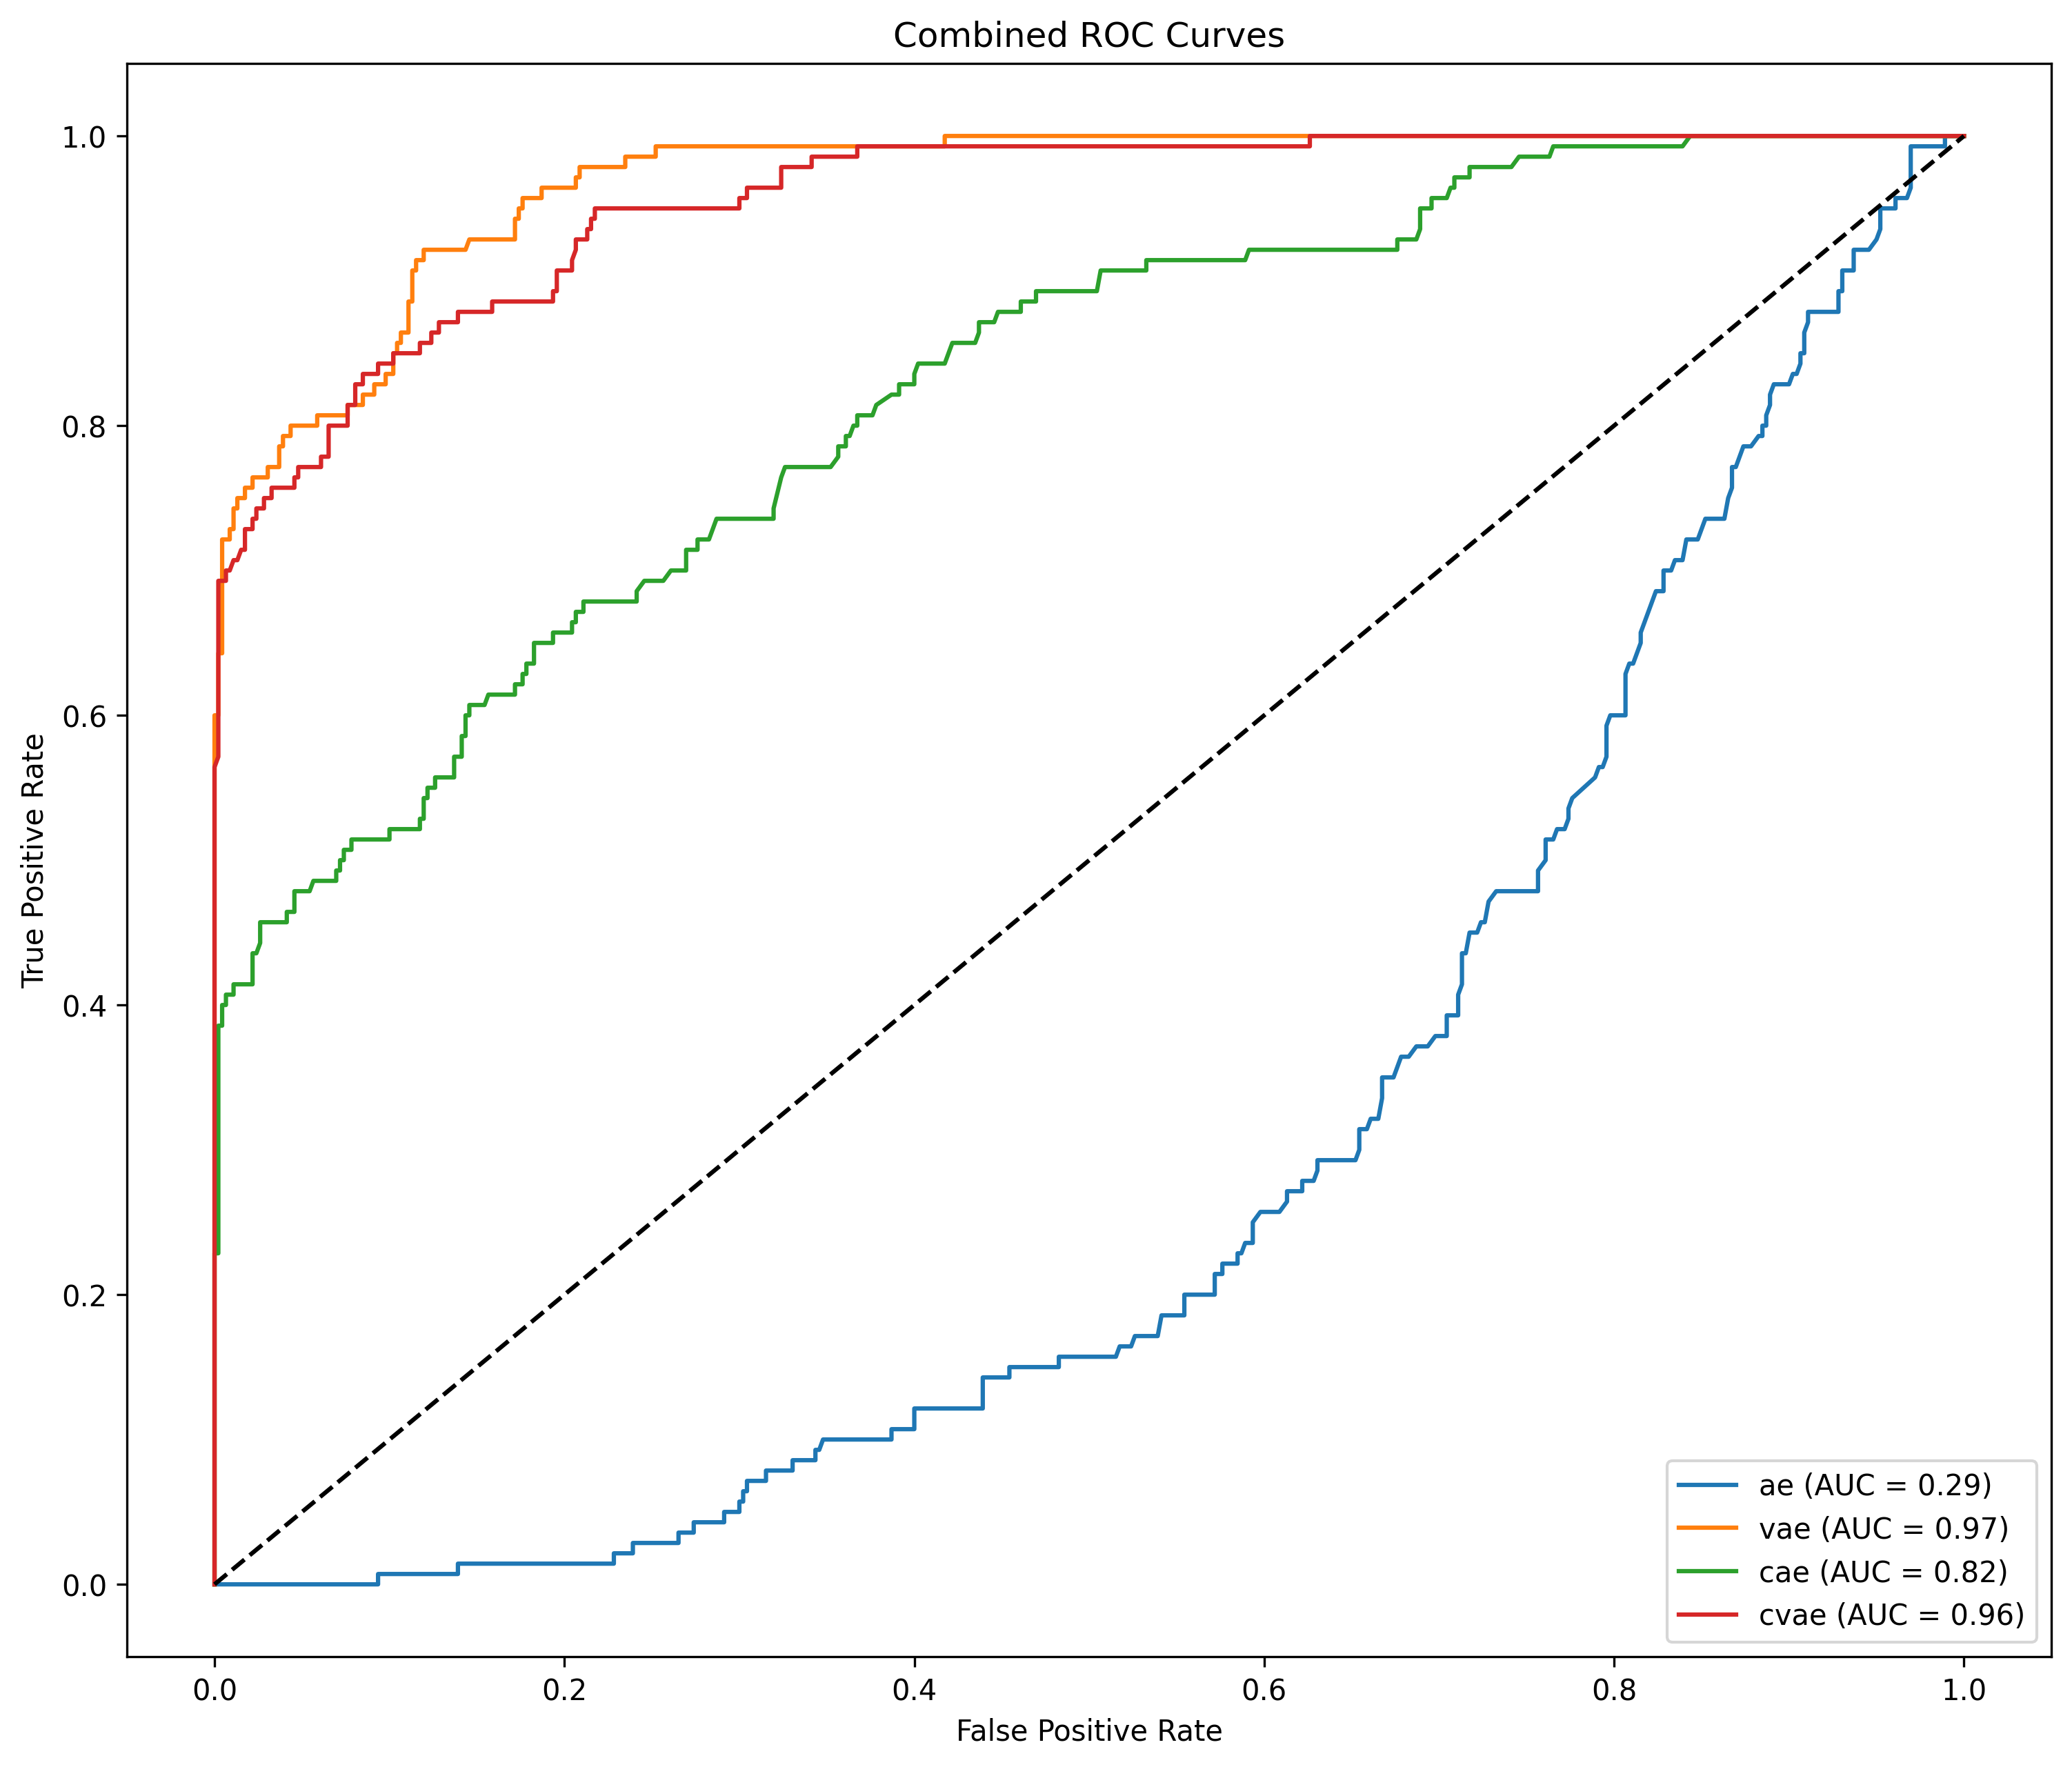
\includegraphics[width=0.7\textwidth]{figures/anomalies/combined_roc_curve.png}
        \caption{Combined ROC Curve for all models using half-precision. AE is Blue, $\beta$-VAE is yellow, CAE is green $\beta$-CVAE is red. The AE model has an upward curve, while the other models perform better, with the variational models yielding high AUC.}
        \label{fig:roccurve}
    \end{subfigure}
    \vspace{1em}
    \begin{subfigure}[b]{\textwidth}
        \centering
        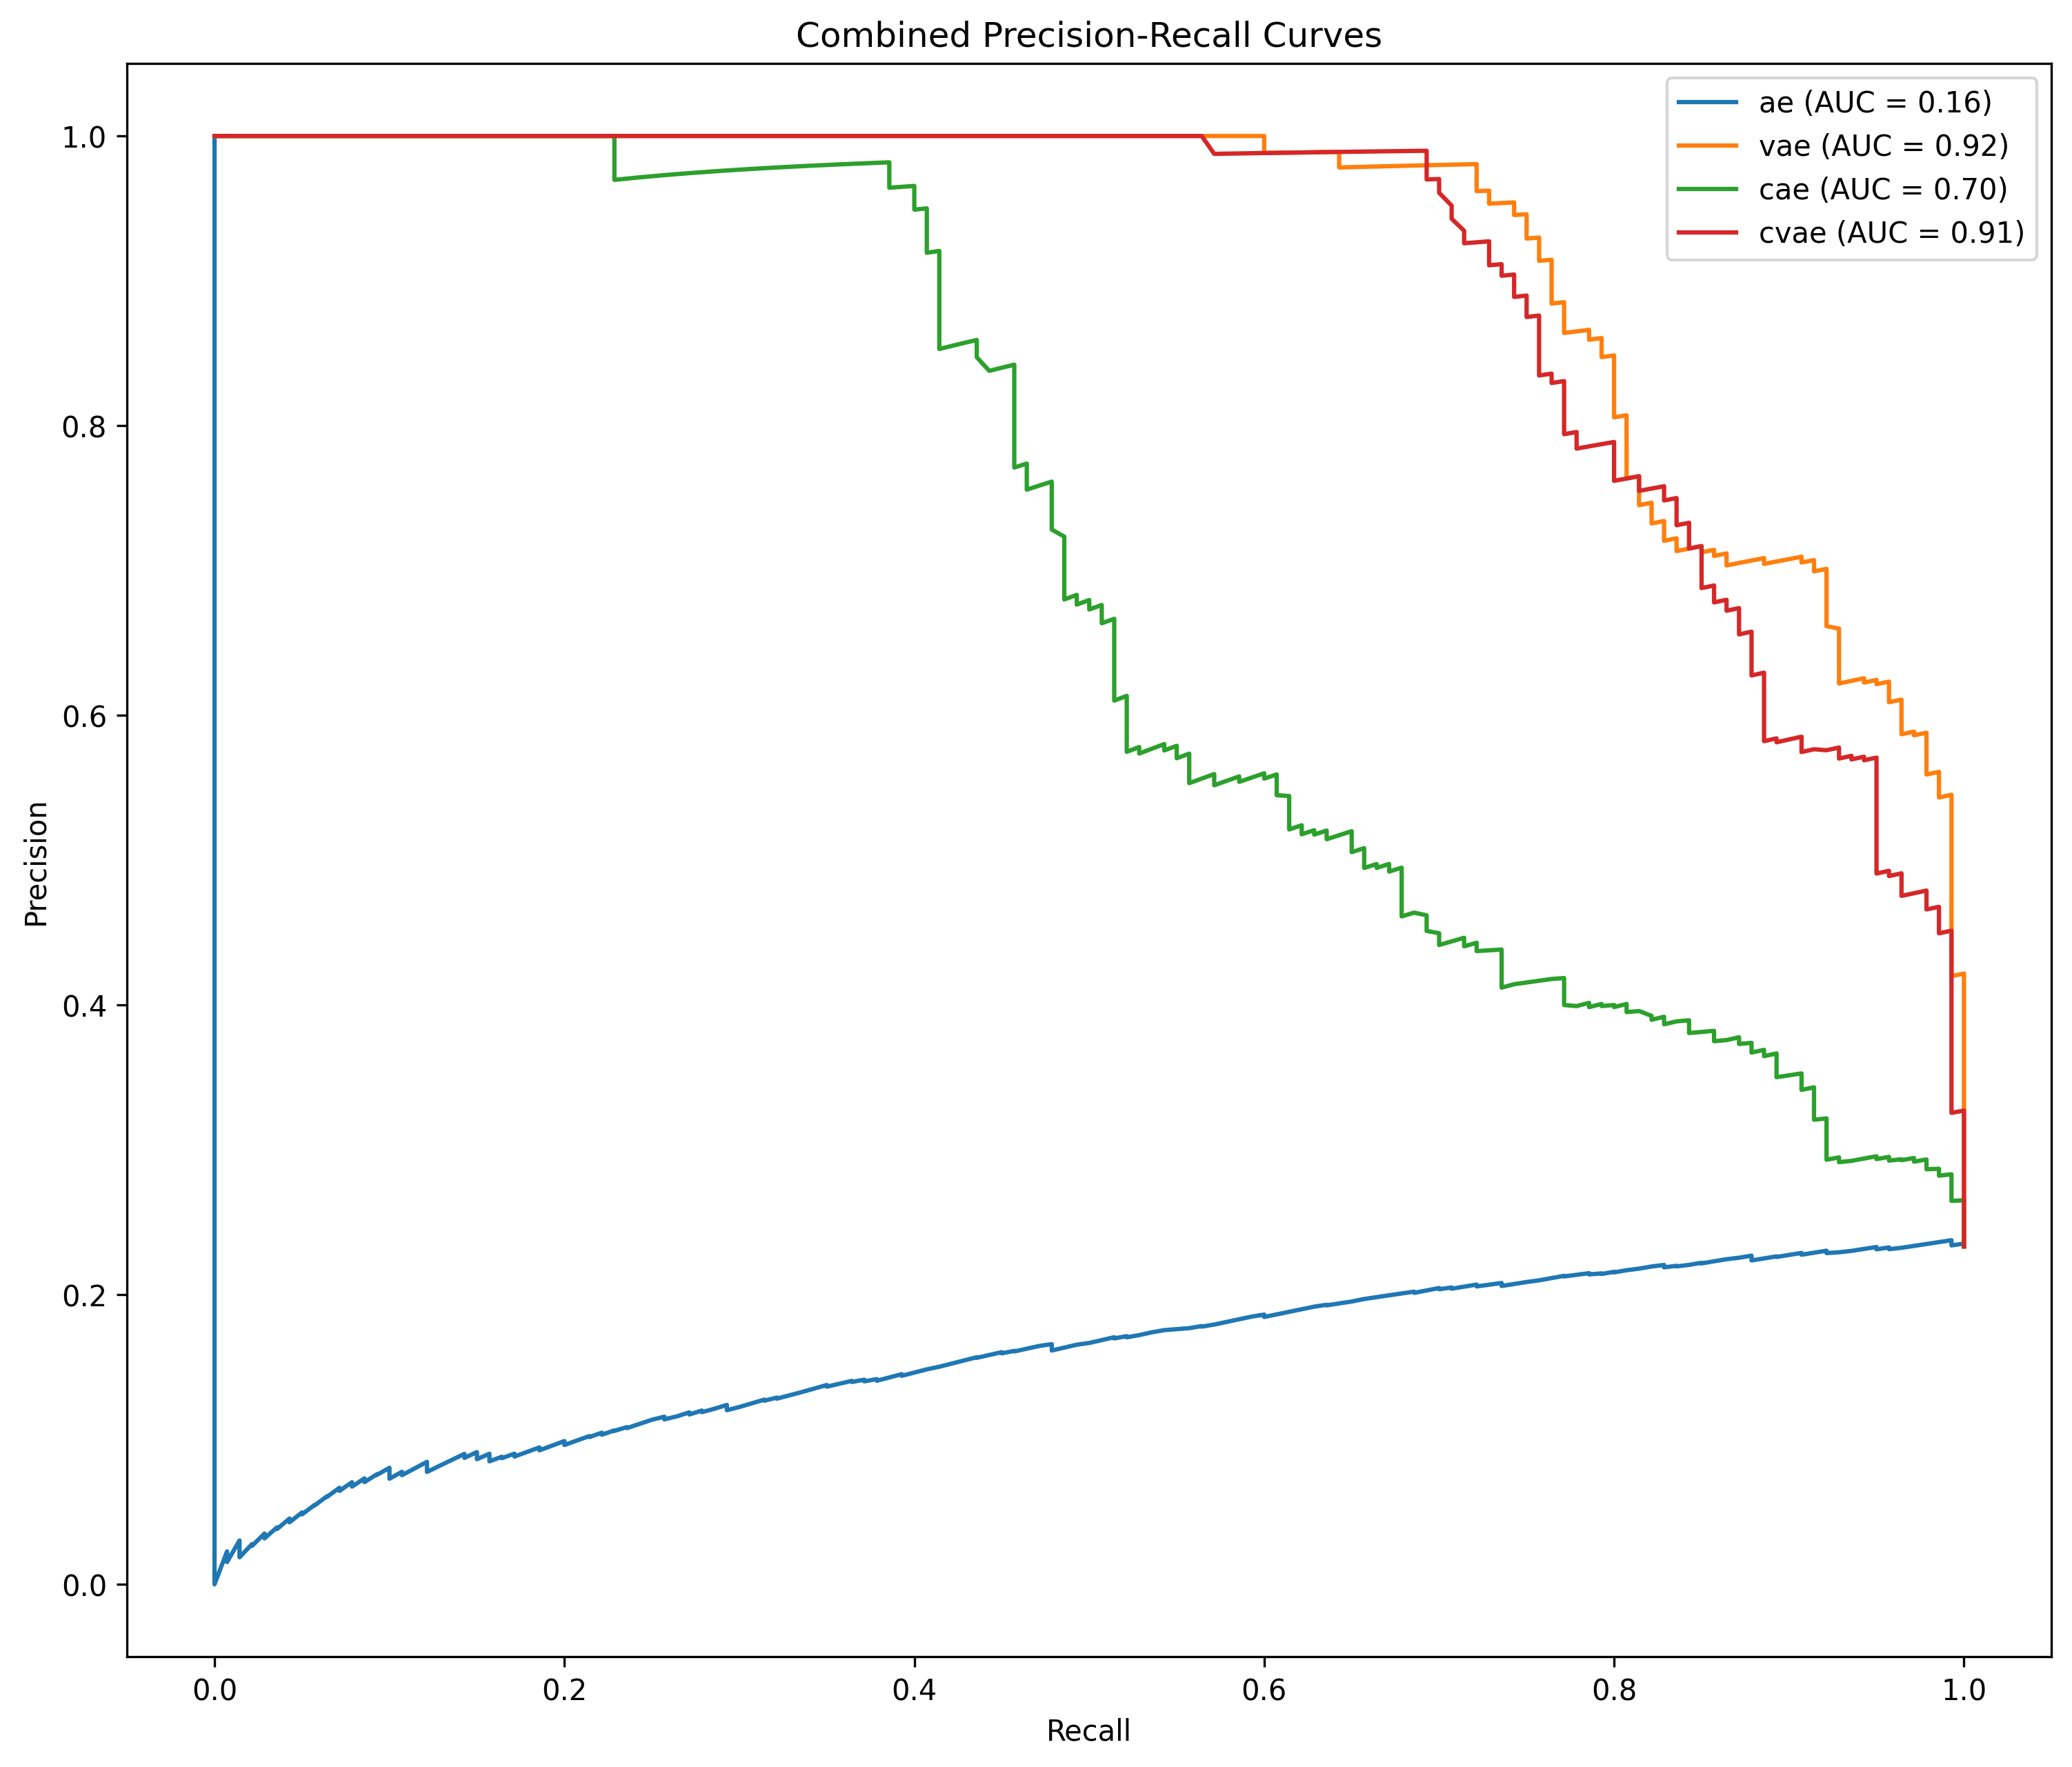
\includegraphics[width=0.7\textwidth]{figures/anomalies/combined_pr_curve.png}
        \caption{Combined PR Curve for all models using half-precision. AE is Blue, $\beta$-VAE is yellow, CAE is green, and $\beta$-CVAE is red. Similar to the ROC curve, The AE model yields the lowest AUC. We also notice }
        \label{fig:prcurve}
    \end{subfigure}
    \label{fig:combined_curves}
\end{figure}
\clearpage

\subsubsection{Threshold Analysis using half-precision inference}

\begin{figure}[!h]
  \centering
  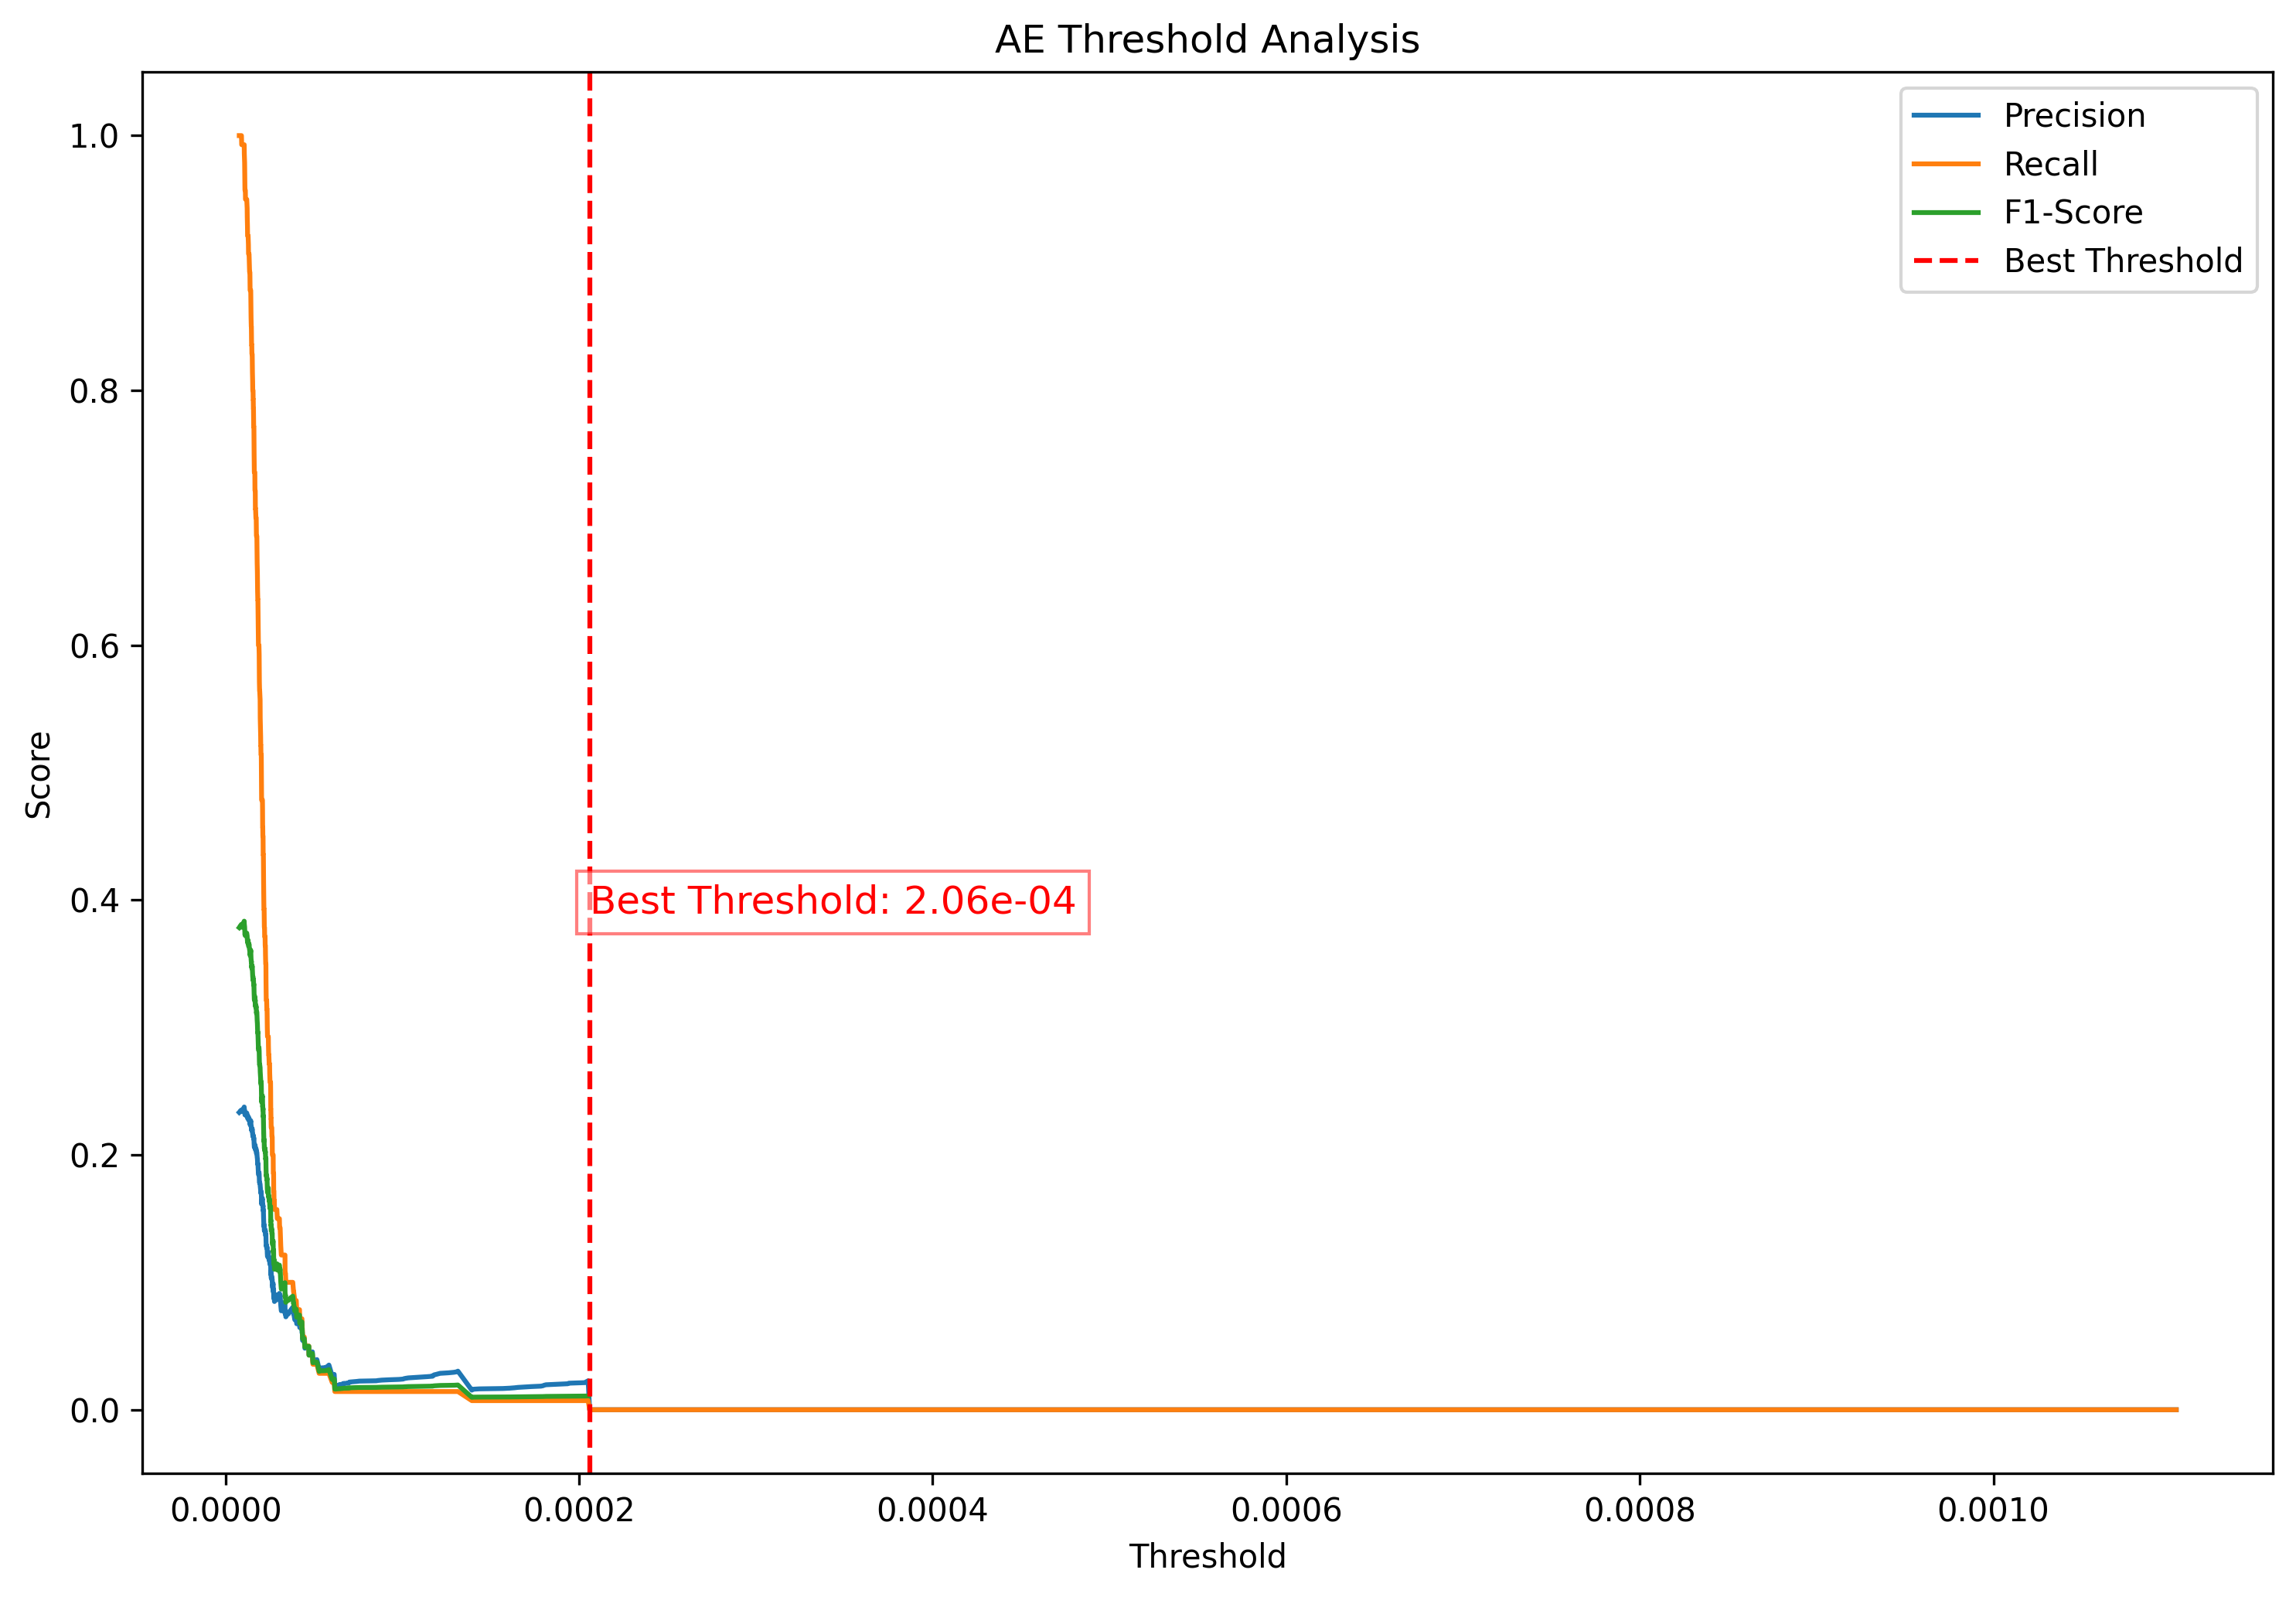
\includegraphics[scale=0.4]{figures/anomalies/ae/threshold_True.png}
  \caption{Threshhold analysis for the AE model. All graphs follow an L-shape structure, with no real peaks for the F1-score. The model still finds a threshold.}
  \label{fig:threshold_ae}
\end{figure}

\begin{figure}[!h]
  \centering
  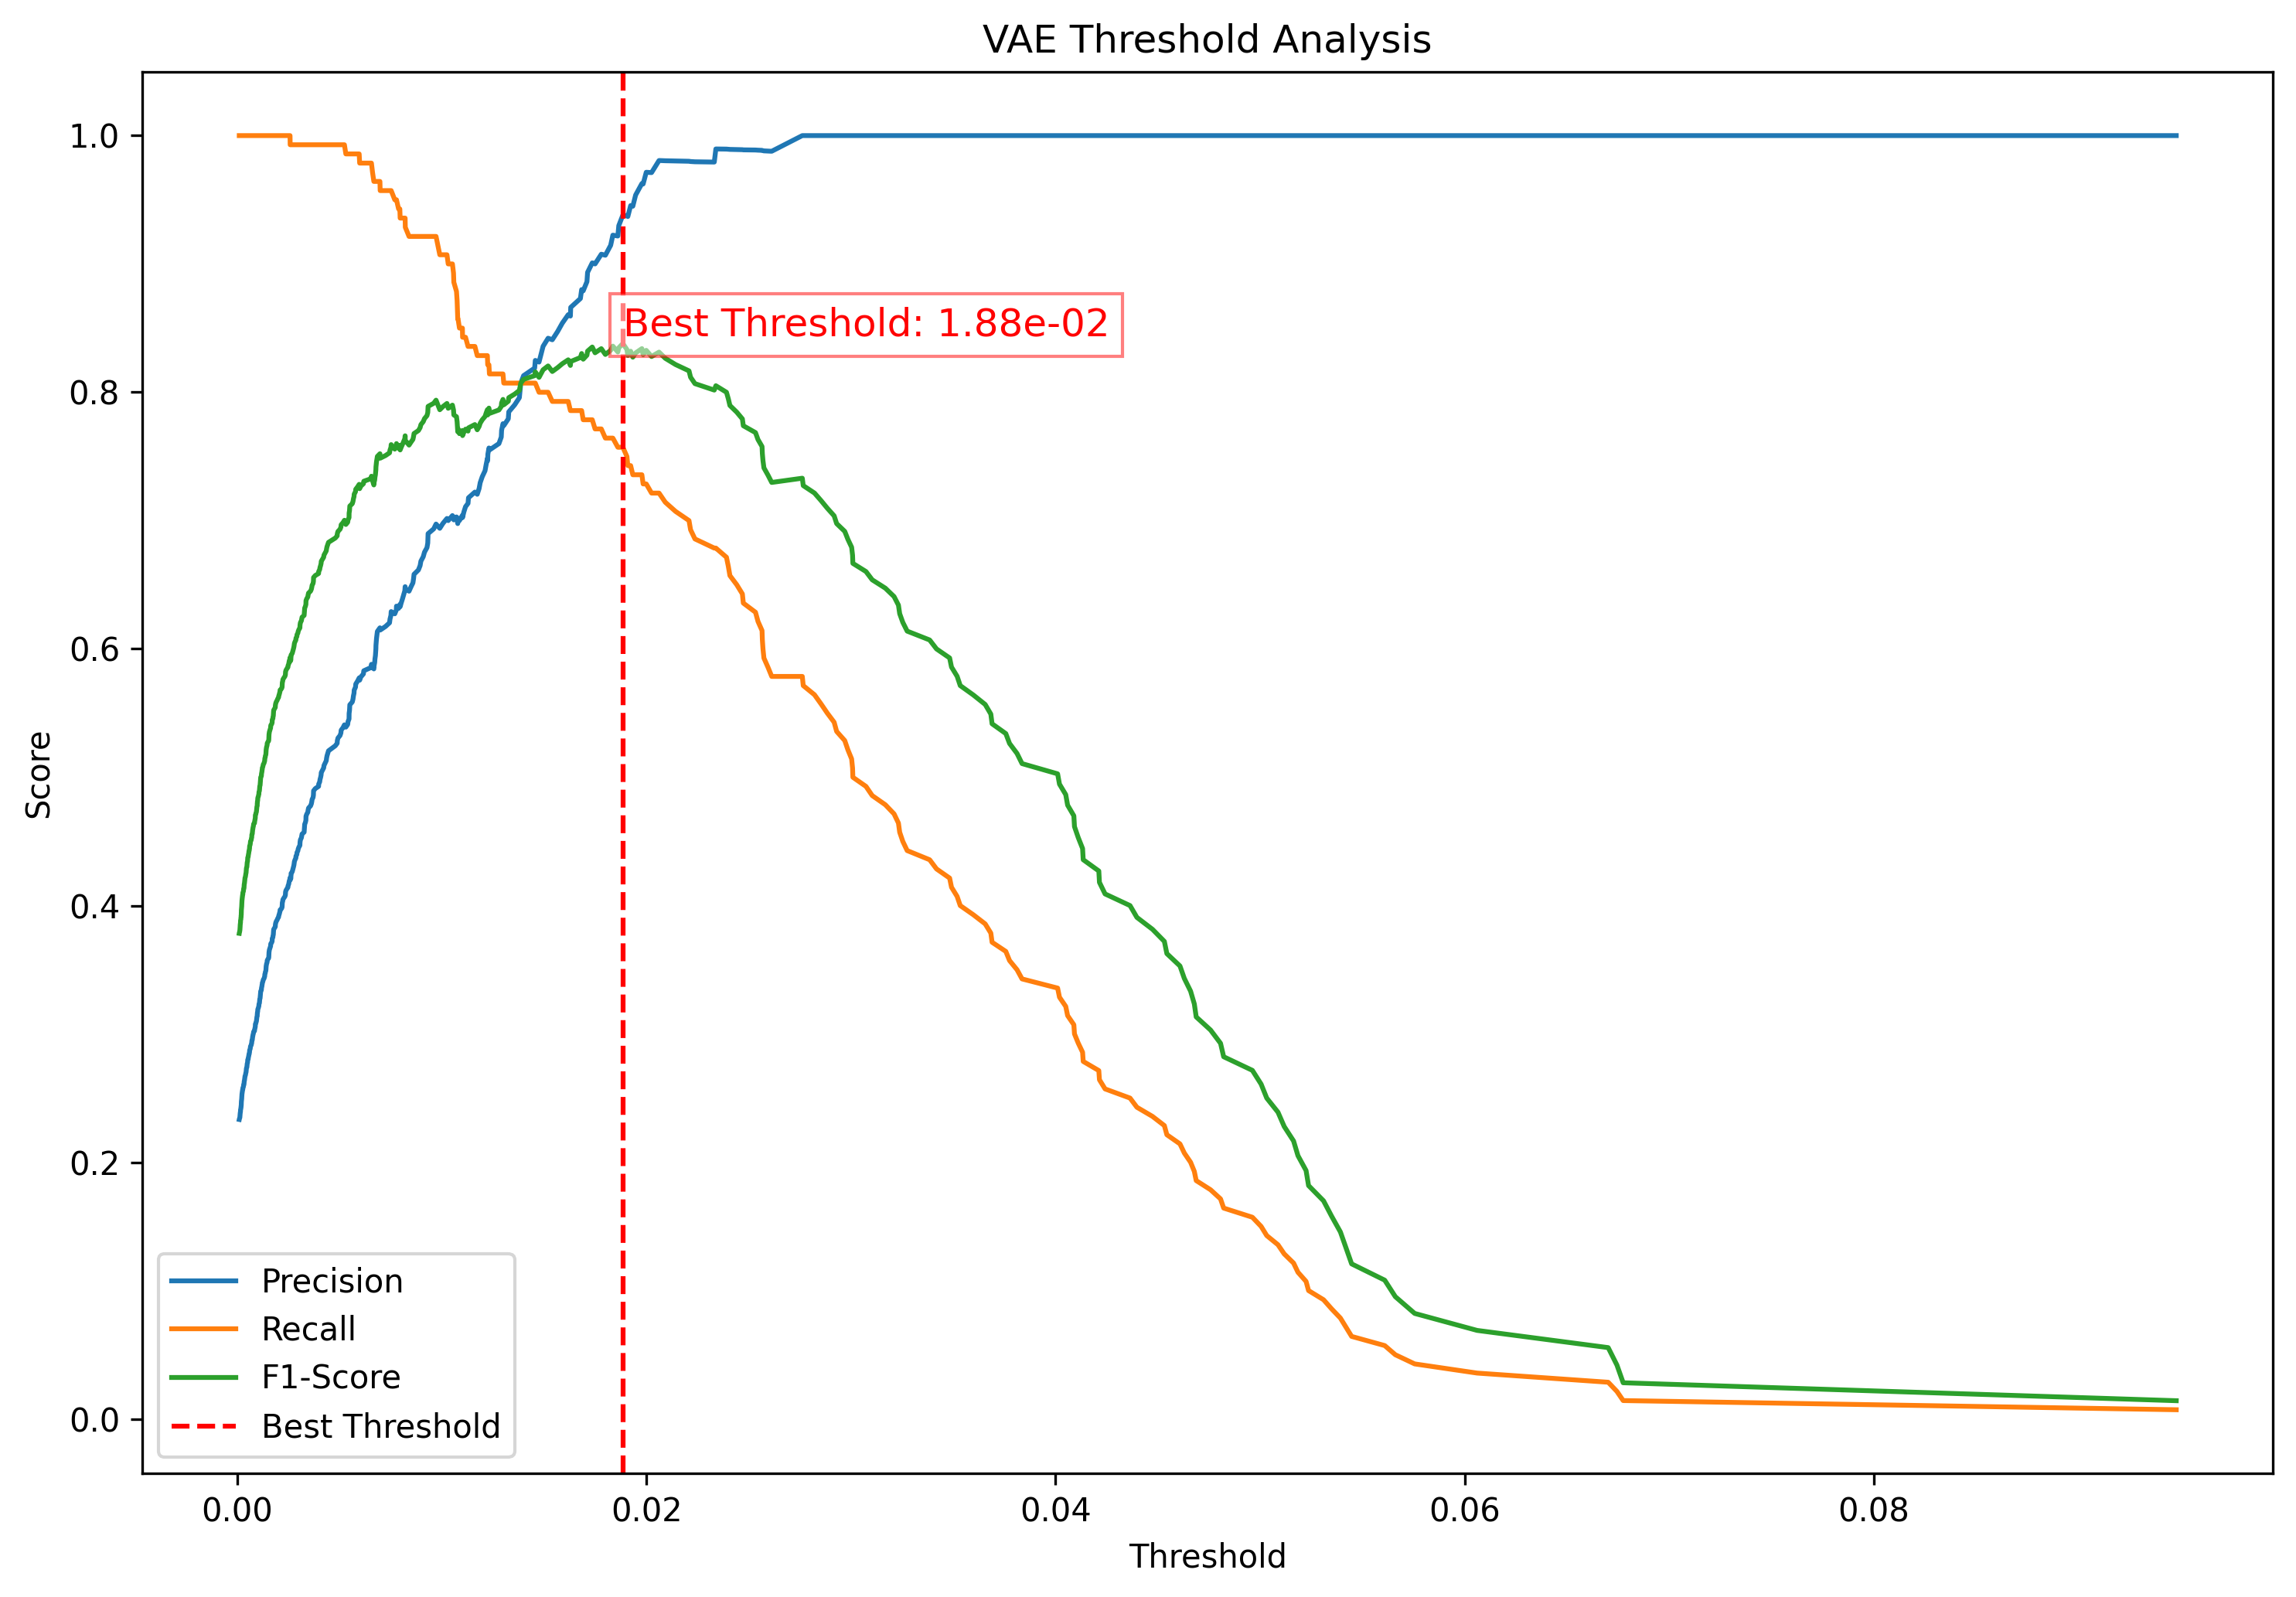
\includegraphics[scale=0.4]{figures/anomalies/vae/threshold_True.png}
  \caption{Threshhold analysis for the $\beta$-VAE model. The threshold found for the $\beta$-VAE models is close to that of AE, but with a distinctive peak in the F1-score.}
  \label{fig:threshold_vae}
\end{figure}

\begin{figure}[!h]
  \centering
  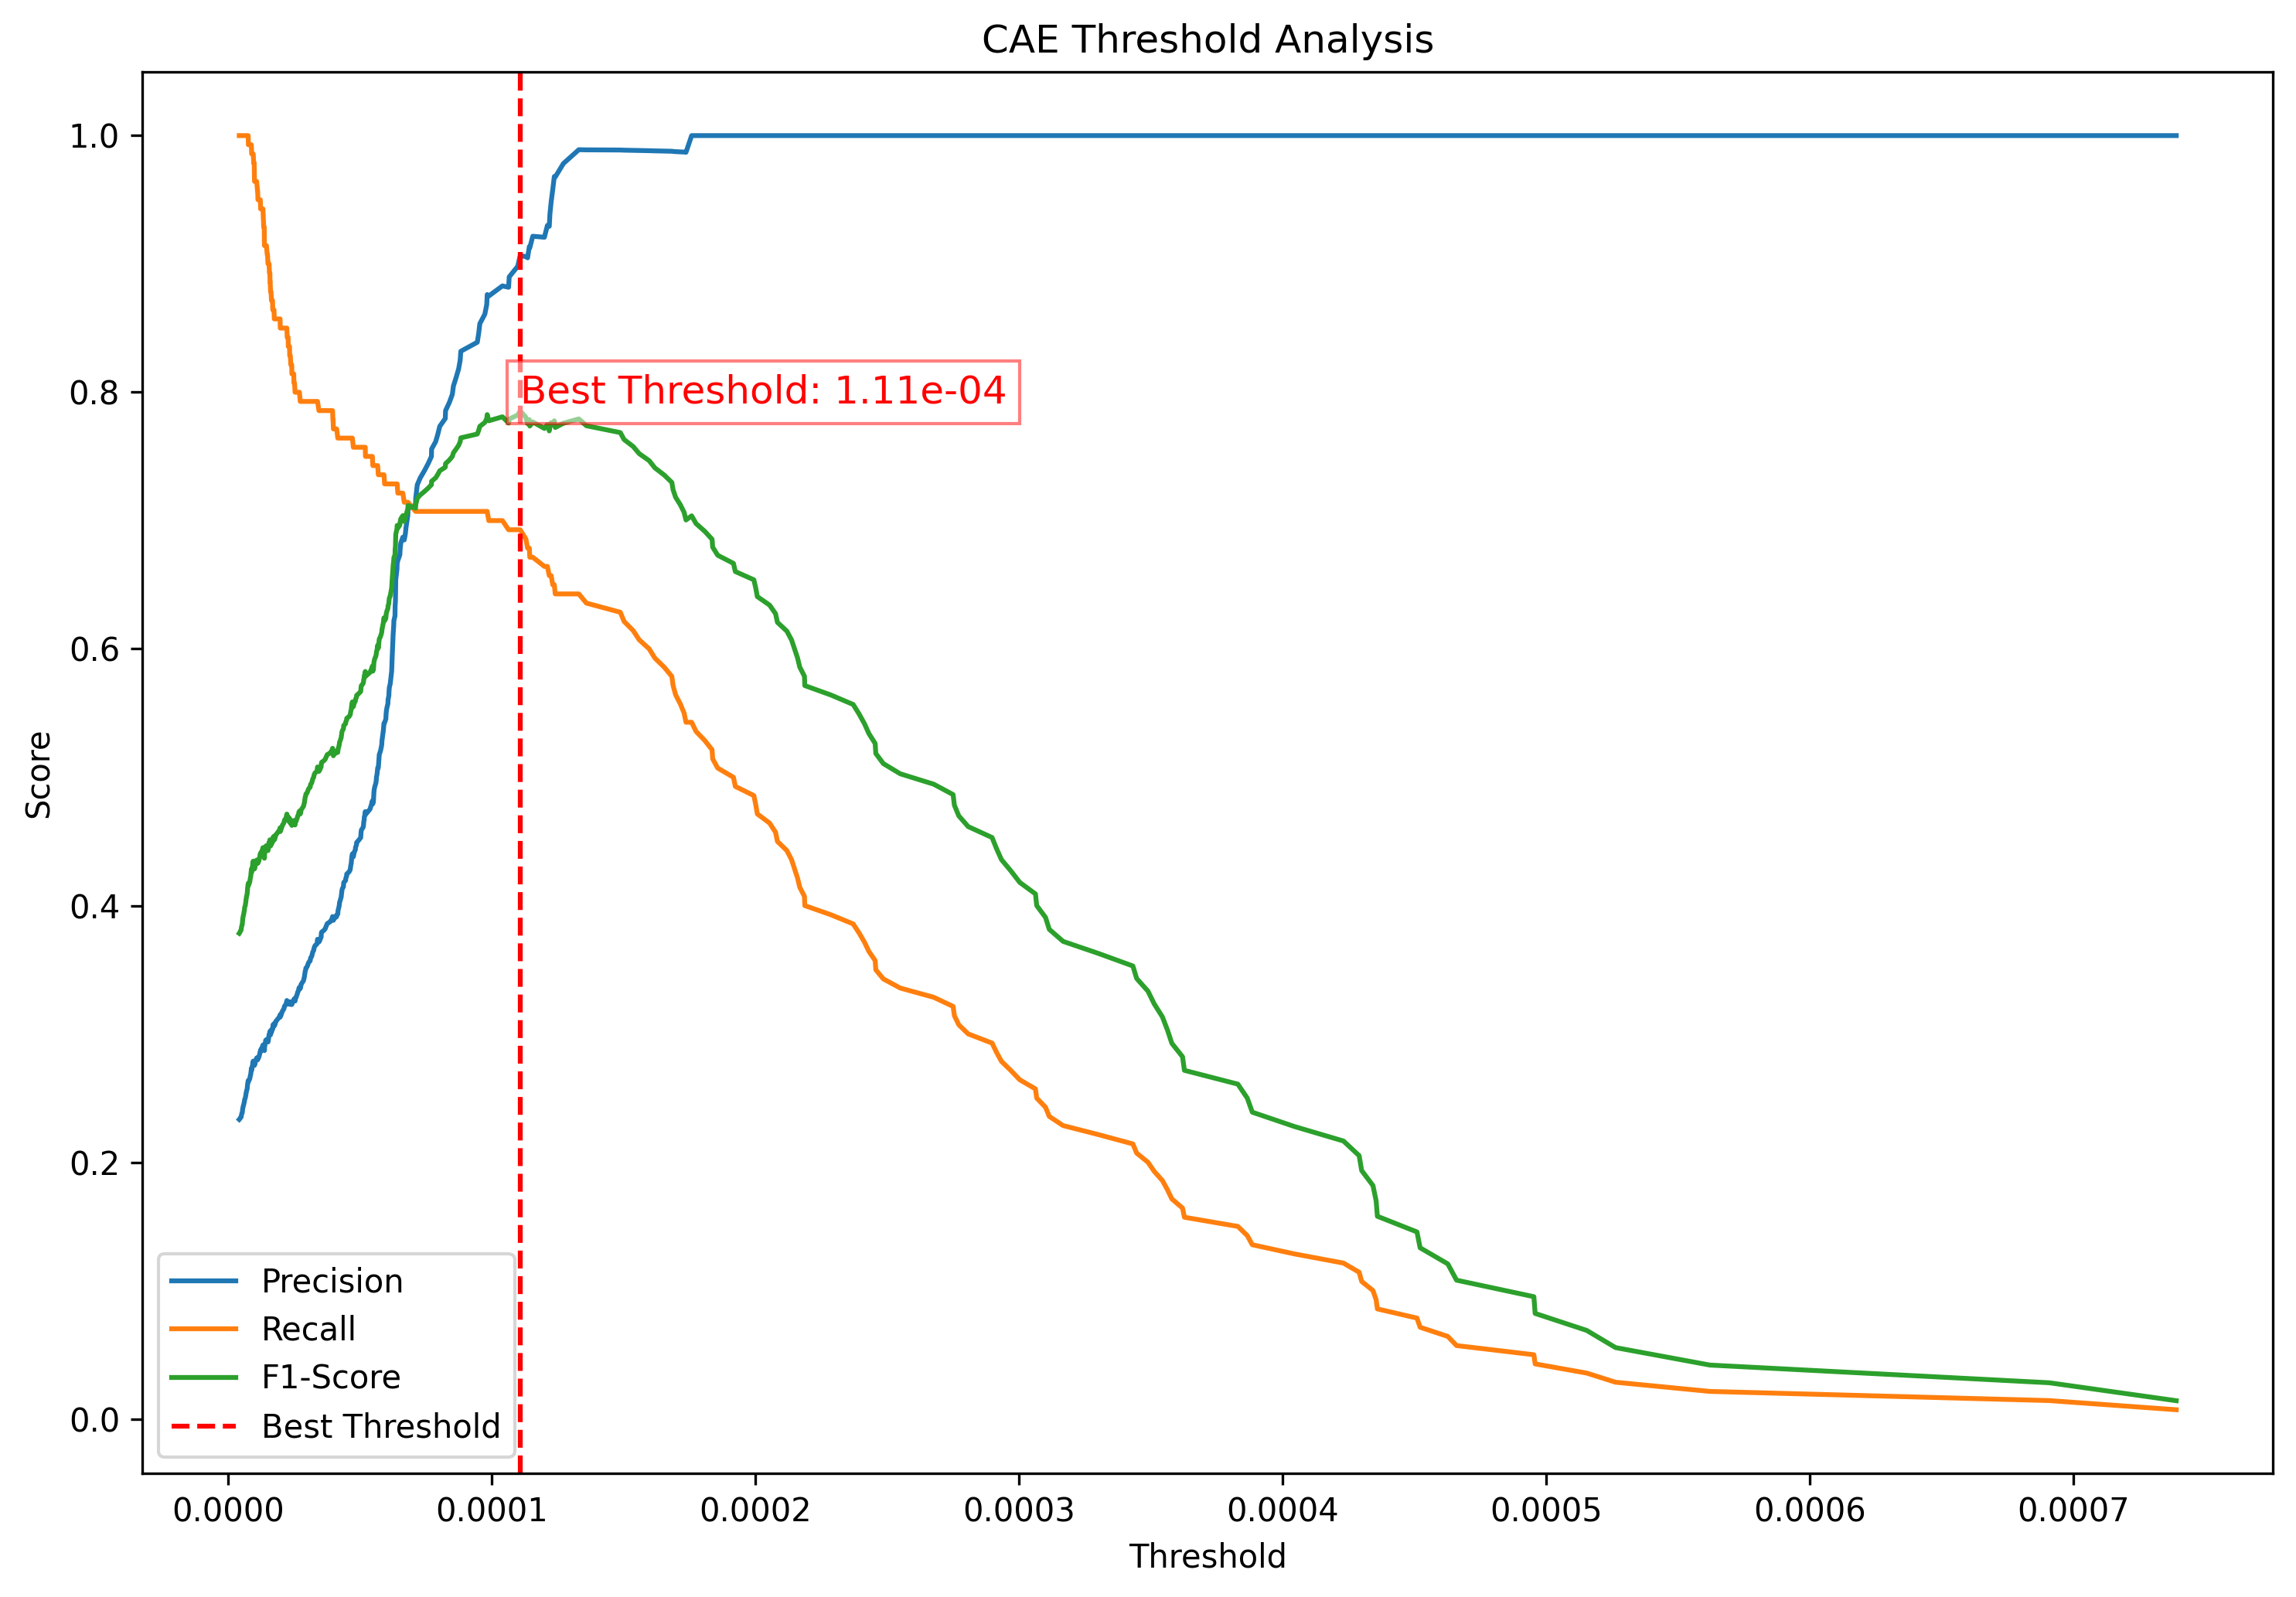
\includegraphics[scale=0.4]{figures/anomalies/cae/threshold_True.png}
  \caption{Threshhold analysis for the CAE model. Its peak is on a different scale compared to the previous models, but the graphs follow the same outline as the one observed in Figure \ref{fig:threshold_vae}.}
  \label{fig:threshold_cae}
\end{figure}

\begin{figure}[!h]
  \centering
  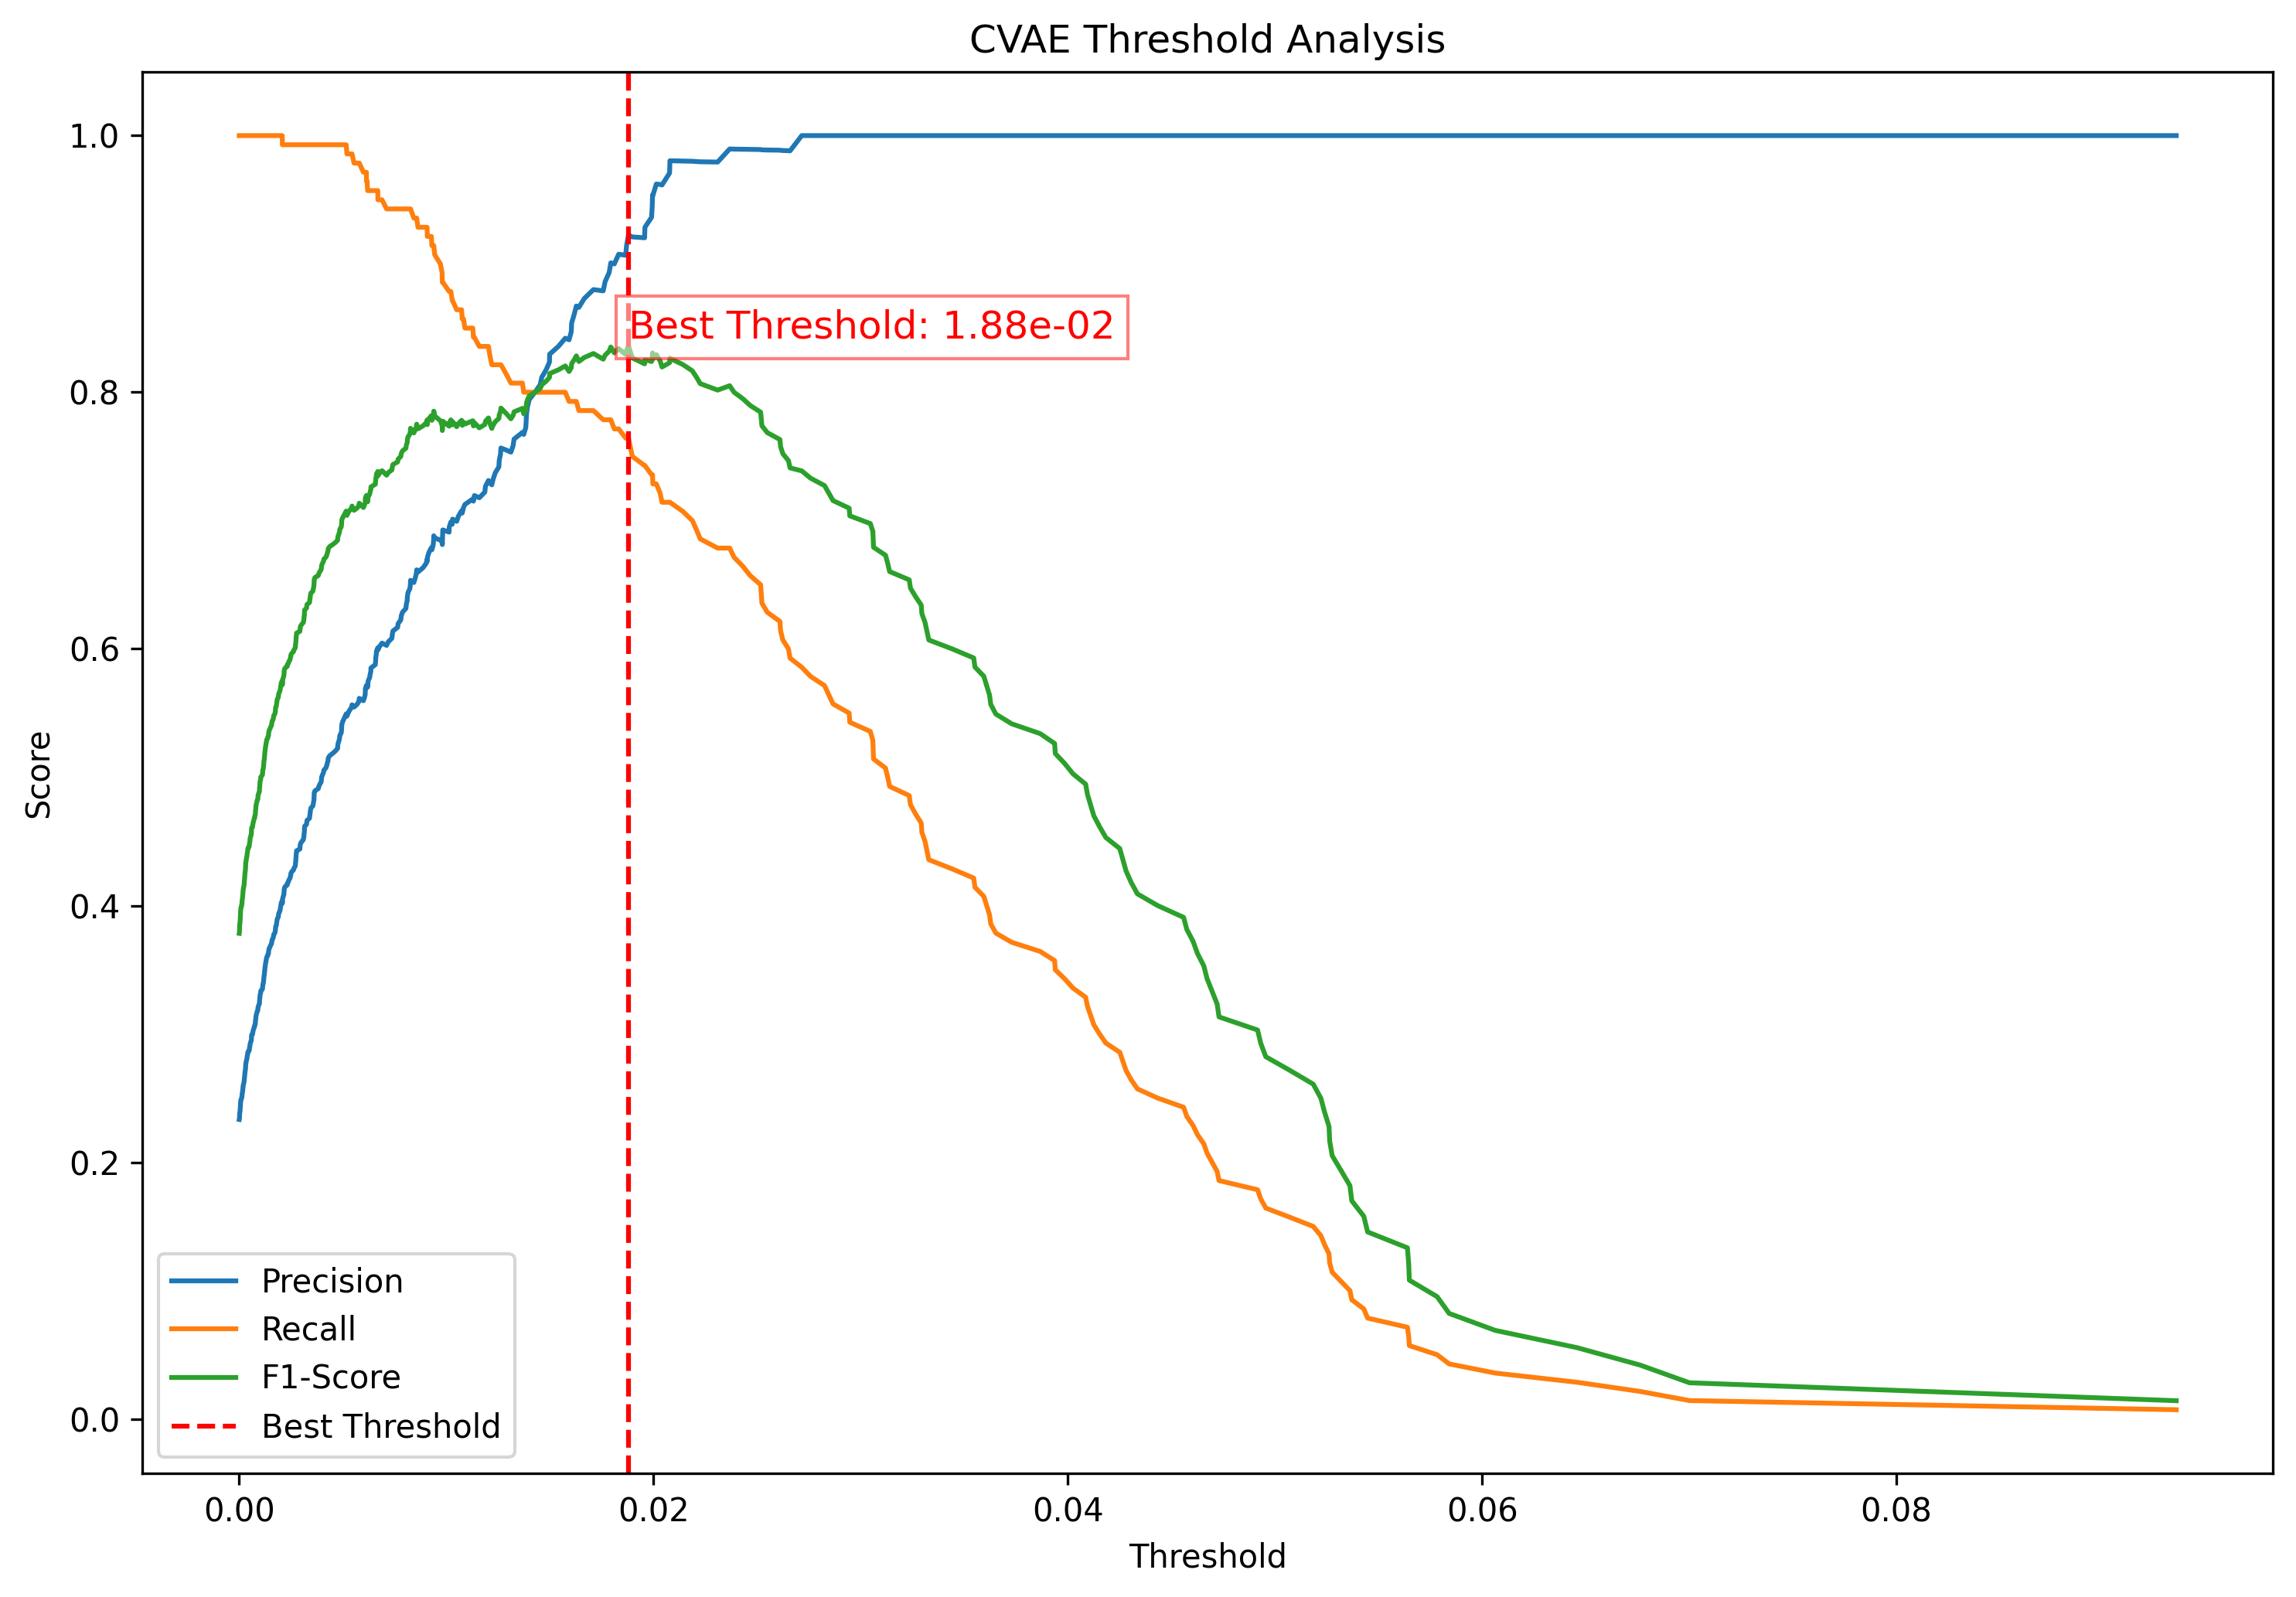
\includegraphics[scale=0.4]{figures/anomalies/cvae/threshold_True.png}
  \caption{Threshhold analysis for the $\beta$-CVAE model. The graphs and best threshold found are close or equal to the ones observed in Figure \ref{fig:threshold_vae}.}
  \label{fig:threshold_vae}
\end{figure}